\documentclass[a4paper,titlepage,12pt]{article}

\usepackage{xcolor}
\usepackage{minted}
\usepackage{amsmath}
\usepackage{titlesec}
\usepackage{graphicx}
\usepackage{bytefield}
\usepackage[portuguese]{babel}
\usepackage[colorlinks=true,allcolors=black,urlcolor=blue]{hyperref}

% Configs
\graphicspath{ {./img/}{./../../../../} }
\newcommand{\sectionbreak}{\clearpage}
\setminted{
    linenos,
    frame=single,
    breaklines,
    fontsize=\small
}

\title{Algoritmos e Estruturas de Dados III\\Prova II}
\author{Fernando de Lima Gonçalves}
\date{Belo Horizonte\\2026}

\begin{document}
\maketitle
\tableofcontents

\section{Compressão}
Para visualização dos métodos de compressão \textit{\sloppy{RLE, Shannon-Fano, Huffman e LZW}} visite: \url{https://solve.vercel.app}.

\subsection{Métodos Estatísticos}

\subsubsection{RLE}
Reduz o tamanho de sequências de símbolos repetidos os substituindo pela quantidade de ocorrencias seguido pelo simbolo.

\begin{figure}[h]
    \centering
    \caption{Compressão RLE}
    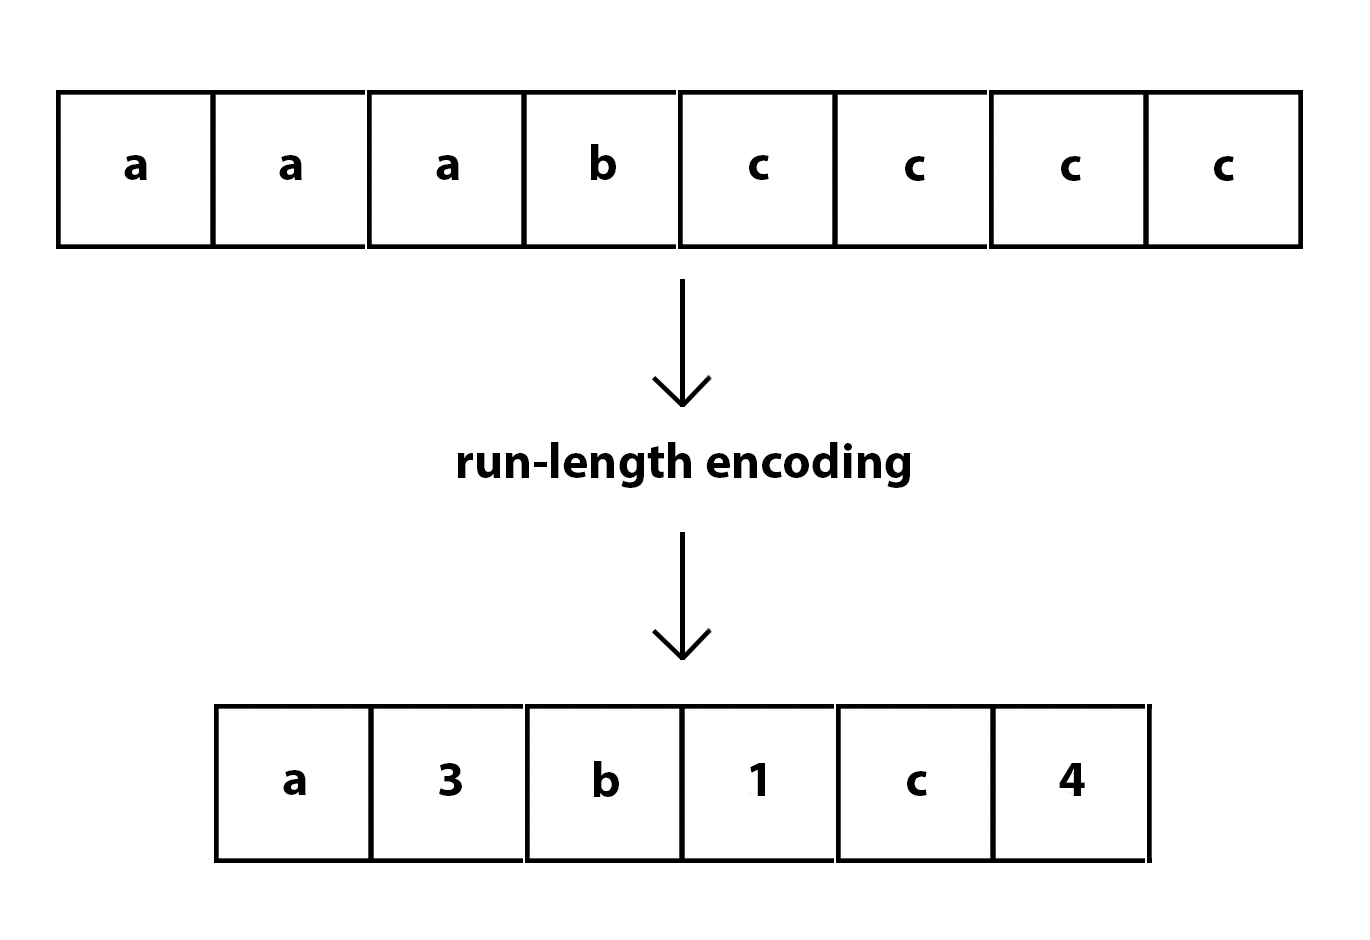
\includegraphics[width=\textwidth]{rle}
    \label{fig:rle}
\end{figure}

\clearpage\subsubsection{Shannon-Fano}
Algoritmo de compressão sem perda desenvolvido por meio de uma arvore binaria \textit{top-down} baseada na probabilidade dos símbolos do conjunto de dados.
A construção da árvore parte da raíz que representa 100\% dos símbolos que se divide, recursivamente, até cada folha representar um único símbolo.
A divisão do grupo de símbolos para os nós filhos busca a igualdade de probabilidade que deve ser avaliado ao executar o algoritmo.
Adotamos para cada caminho para esquerda entre nós esquerda como 0 e para direita como 1 para obter um valor binário de n-bits, onde n é a altura da folha.

\begin{figure}[h]
    \centering
    \caption{Compressão Shannon-Fano}
    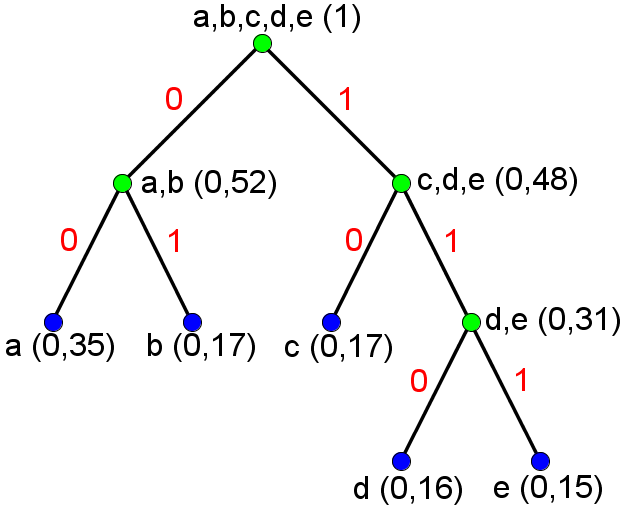
\includegraphics[width=\textwidth]{tree-sf}
    \label{fig:Shannon-Fano}
\end{figure}

\clearpage\subsubsection{Huffman}
Algoritmo de compressão sem perda muito similar a Shannon-Fano porém com construção da árvore \textit{botton-up} garantindo resultados ótimos.
\sloppy{Caminhamento e atribuição de valores segue mesmo padrão de Shannon-Fano atribuindo 0 para esquerda e 1 para direita e obter valores binários para
os símbolos.}

\begin{figure}[h]
    \centering
    \caption{Compressão Huffman}
    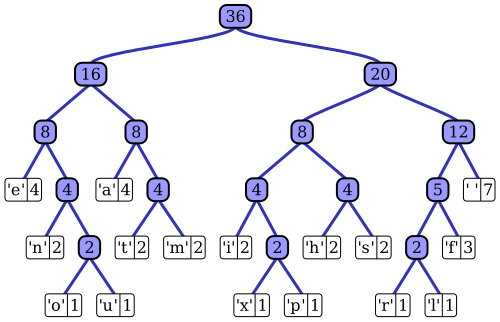
\includegraphics[width=\textwidth]{tree-huf}
    \label{fig:Huffman}
\end{figure}

\clearpage\subsection{Métodos de Dicionário}
\subsubsection{LZ77}
Método de compressão que utiliza o conceito de \textit{\textbf{janela deslizante}}.

\begin{figure}[h]
    \centering
    \caption{Compressão LZ77}
    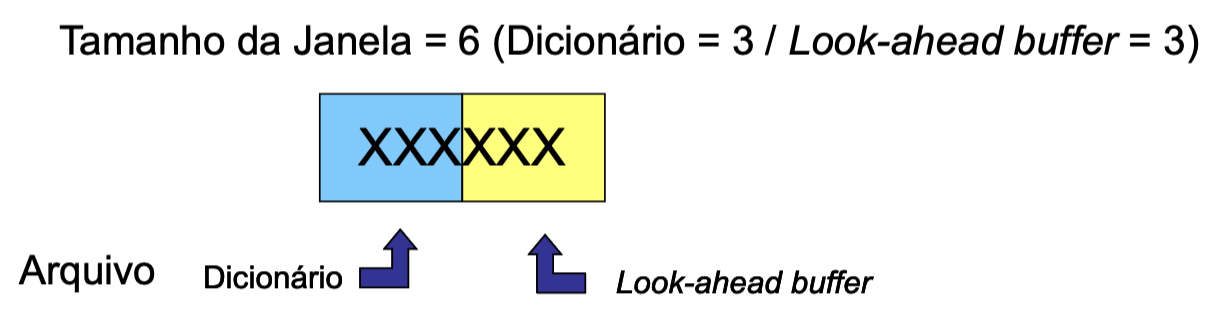
\includegraphics[width=\textwidth]{lz77}
    \label{fig:LZ77}
\end{figure}

\clearpage\subsubsection{LZ78}

\begin{figure}[h]
    \centering
    \caption{Compressão LZ78}
    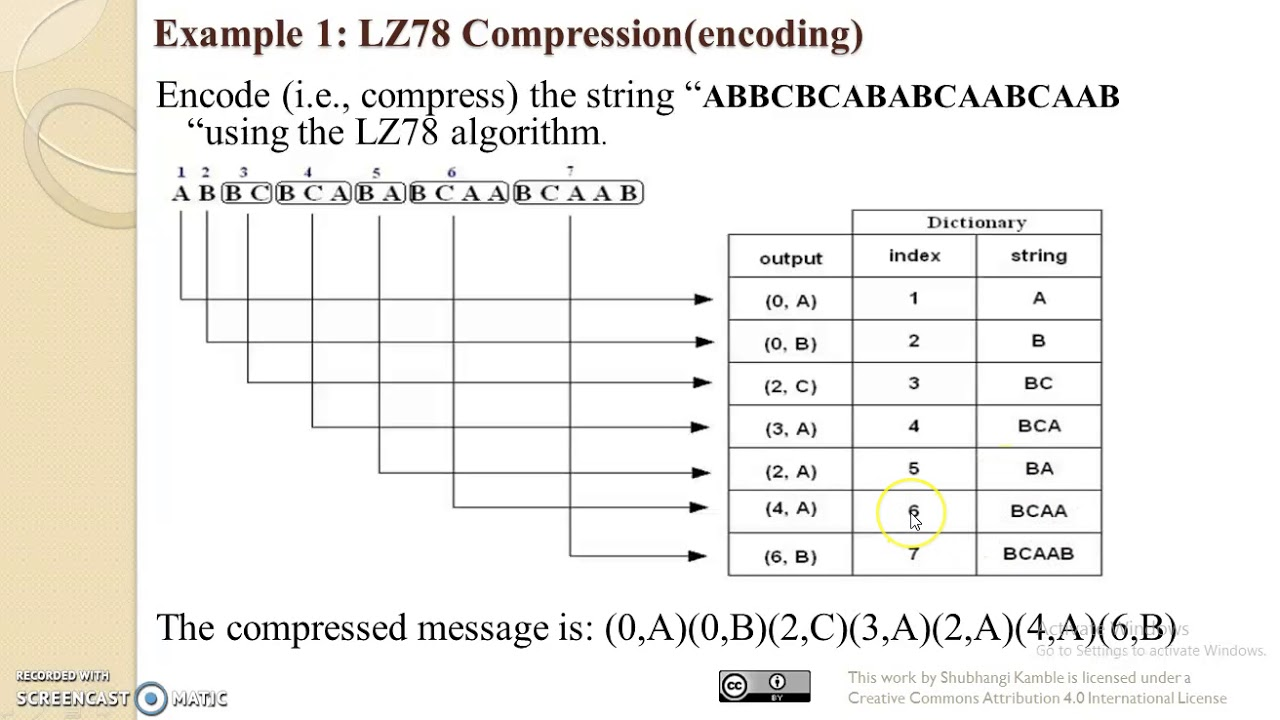
\includegraphics[width=\textwidth]{lz78}
    \label{fig:LZ78}
\end{figure}

\clearpage\subsubsection{LZW}

\section{Casamento de Padrões}
\subsection{Força Bruta}

\subsection{KMP}

\subsection{Boyer-Moore}

\subsection{Shift-AND}

\subsection{Rabin-Karp}

\subsection{Aho Corasick}

\subsection{Levenshtein}
\end{document}
